\section{Geometric and Negative Binomial Distributions}
\subsection{The Geometric Distribution}

The geometric distribution models the number of independent Bernoulli trials needed to get the first success. If each trial has probability of success $p$ and probability of failure $q=1-p$, then the random variable $X$ that counts the number of trials up to and including the first success has probability function
\begin{align}
 \label{eq:2.10.9}
 f(k) = P(X=k) = (1-p)^{k-1}p, \quad k=1,2,3,\dots
\end{align}

A fundamental property of the geometric distribution is \emph{memorylessness}: the probability of obtaining a success in the next $k$ trials does not depend on the number of previous failures. That is, if $m,n\geq 1$,
\begin{align}
 P(X > m+n \mid X > m) = P(X > n).
\end{align}

{Properties of the geometric distribution} If $X$ has a geometric distribution with parameter $p$, then
\begin{align}
 \mu_{X} &= \dfrac{1}{p} \\
 \s_{X}^{2} &= \dfrac{1-p}{p^{2}}.
\end{align}

\begin{ejemplo}
 \label{exmp:2.10.13}
 A salesperson knows that the probability of closing a sale on any given telephone call is $p=0.2$. What is the probability that they need to make exactly $5$ calls to make the first sale? How many calls are expected on average?
\end{ejemplo}

\begin{solucion}
	Using the geometric distribution with $p=0.2$:
	\begin{align}
		P(X=5) &= (1-0.2)^{5-1}(0.2) = (0.8)^{4}(0.2) \\
		&= 0.4096 \times 0.2 = 0.08192
	\end{align}

	The expected number of calls is
	\begin{align}
		\mu = \dfrac{1}{p} = \dfrac{1}{0.2} = 5.
	\end{align}
\end{solucion}

\begin{ejemplo}
 \label{exmp:2.10.14}
 In a quality control process, the probability that a part is defective is $p=0.1$. What is the probability that the first defective part appears on the third inspection?
\end{ejemplo}

\lstinputlisting[language=Python]{../code/distribuciones-especiales/distGeom.py}

\begin{figure}
 \centering
 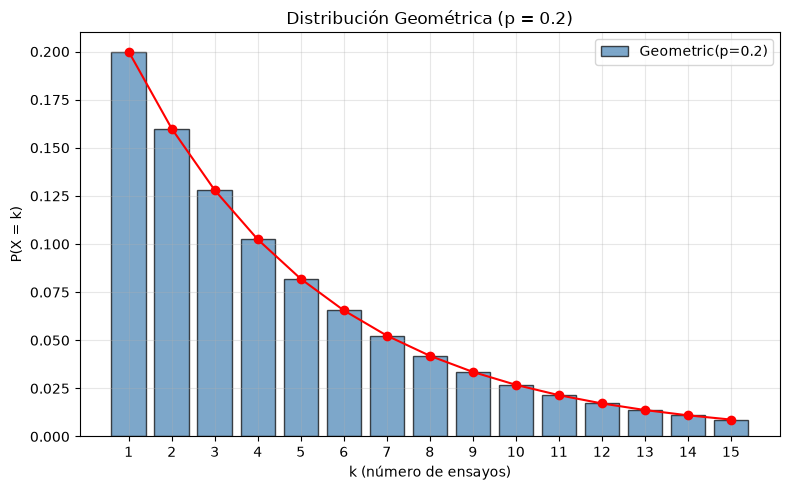
\includegraphics[height=7cm,keepaspectratio=true]{./pe/distGeom.png}
 % distGeom.png: 0x0 pixel, 300dpi, 0.00x0.00 cm, bb=
 \caption{Geometric distribution with $p=0.2$}
 \label{fig:2.10.7}
\end{figure}

\subsection{The Negative Binomial Distribution}

The negative binomial distribution generalizes the geometric distribution: it models the number of failures observed before obtaining a predetermined number $r$ of successes in a sequence of independent Bernoulli trials. Its probability function is given by
\begin{align}
 \label{eq:2.10.10}
 f(k) = P(X=k) = \binom{k+r-1}{r-1}p^{r}(1-p)^{k}, \quad k=0,1,2,\dots
\end{align}

Note that when $r=1$, the negative binomial reduces to the geometric distribution (counting failures before the first success).

{Properties of the negative binomial distribution} If $X$ has a negative binomial distribution with parameters $r$ and $p$, then
\begin{align}
 \mu_{X} &= \dfrac{r(1-p)}{p} \\
 \s_{X}^{2} &= \dfrac{r(1-p)}{p^{2}}.
\end{align}

\begin{ejemplo}
 \label{exmp:2.10.15}
 A certification exam has a pass rate of $30\%$. What is the probability that a student fails $4$ times before passing for the third time?
\end{ejemplo}

\begin{solucion}
	In this case, $r=3$ (number of successes) and $p=0.3$. The variable $X$ counts the number of failures before the third success.
	\begin{align}
		P(X=4) &= \binom{4+3-1}{3-1}(0.3)^{3}(0.7)^{4} \\
		&= \binom{6}{2}(0.027)(0.2401) \\
		&= 15 \times 0.027 \times 0.2401 \\
		&\approx 0.0972
	\end{align}
\end{solucion}

\lstinputlisting[language=Python]{../code/distribuciones-especiales/distNegBinom.py}

\begin{figure}
 \centering
 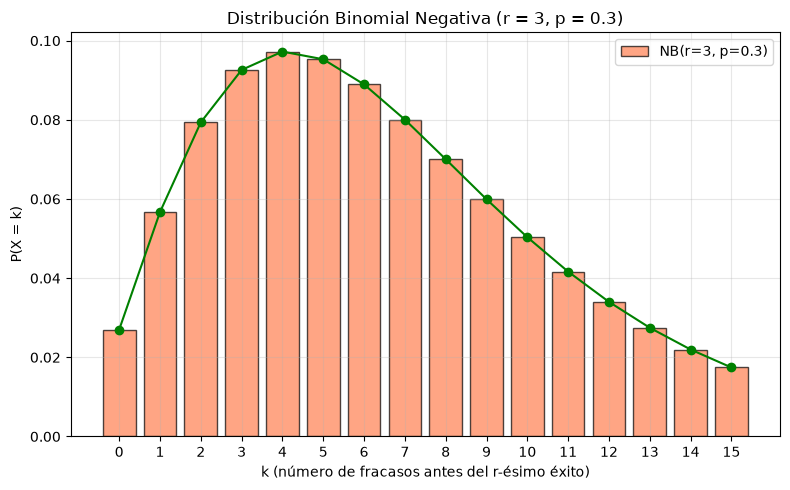
\includegraphics[height=7cm,keepaspectratio=true]{./pe/distNegBinom.png}
 % distNegBinom.png: 0x0 pixel, 300dpi, 0.00x0.00 cm, bb=
 \caption{Negative binomial distribution with $r=3$, $p=0.3$}
 \label{fig:2.10.8}
\end{figure}
